\chapter{Planeación}
\section{Planteamiento del Problema}

El problema consiste en que al momento de realizar inventarios se hace necesario llevar a cabo un conteo de las unidades para anotarlas en un cuderno, de igual manera restar las unidades vendidas dependiendo el producto y posteriormente este sera el valor numerico que se encuentra en stock.

Por otra parte se necesitaba hacer diario un inventario de ventas y de productos, con la necesidad de que este no se podia acumular por que si se dejaba de hacer por unos dias se convertia en una lista de productos que debian salir del inventario causando errores.


\section{Justificación}

Es valido resolver este problema debido a que con esta solucion de software se podra realizar inventario mensual, semanal y diario con una sola tirilla de productos y sus totales vendidos, de igual forma ya no sera necesario la facturacion a mano disminuyendo el uso de papel y el porcentaje de error debido a trabajo humano.

Por otra parte se pueden observar con menor dedicacion de tiempo parametros como ventas diarias, semanales, mensuales, las cuales se revisan para plantear metas y otros parametros como ventas por usuario las cuales pueden proporcionar informacion de rendimientos.


\section{Objetivos}
\subsection{Objetivo General}

Diseñar y desarrollar un prototipo de software basado en java para llevar contabilidad y inventario en un almacén.

\subsection{Objetivos Específicos}
\begin{itemize}
    \item Desarrollar una aplicacion de escritorio con el cual se puedan llevar los inventarios y ventas de un almacen.
    \item Implementar el patron MVC.

\end{itemize}

\section{Alcances}

El proyecto podra ofrecer un aplicativo editable para diferentes tipos de clientes, es decir, diferentes almacenes. Cada aplicativo tendra la posibilidad de llevar modulos segun el cliente los solicite y ser editado al estilo del almacén.

Asimismo se podran agregar modulos con facilidad para generar nuevas soluciones para requerimientos a peticion del cliente.



\section{Limitaciones}

El proyecto prestara unicamente soluciones para empresas basadas en productos de venta libre, manejo de facturacion e inventario, no se podran acceder a estos de manera remota, ni prestara un servicio de impresión.

\subsection{Marco Metodológico}

La metodología  \textit{SCRUM}  es un proceso de desarrollo de software con metodologia agil y flexible. Su principal objetivo es maximizar la inversion y disminuir el tiempo de desarrollo. 

Este proceso permite entregar cada fin de la iteracion un prototipo funcional y crear espectativas para cada iteracion. Esta metodologia permite obtener los siguientes beneficios. 

\begin{enumerate}

    \item \textbf{Cumplimento de expectativas:} Esta metodologia permite que el cliente genere unas espectativas y el arquitecto de scrum planea cada iteracion y genera prioridades.
    
    \item \textbf{Flexibilidad a cambios:} Esta metodologia presenta una alta capacidad al cambio especialmente en los requerimientos.
    
    \item \textbf{Reducción del Time to Market:} Se le puede dar uso a los diferentes prototipos y se puede entregar un prototipo parcial para realizar su evaluacion.
    
    
\end{enumerate}

La Tabla \ref{table:Actividades-durante-un-sprint-de-scrum} presenta las diferentes actividades realizadas con base en las fases de la metodología RUP.

\begin{center}
\begin{longtable}{|c|l|p{6.5cm}|p{8.5cm}|}
\caption{Actividades durante un Sprint de SCRUM}
\label{table:Actividades-durante-un-sprint-de-scrum}
\\ \hline
\textbf{Etapa}&\textbf{Actividad}&\textbf{Descripción} \\ \hline
\multirow{10}{*}{\rotatebox{90}{Planeamiento del sprint}} 
    & \multirow{1}{*}{Planeacion del sprint}
        & Durante la planeacion del sprint se llaman a renunion todos los participantes del equipo, durante la consecucion de este evento se decide que requerimientos o actividades van a ser asignados a los integrantes. Cada integrante debera asignar un elemento de tiempo en el cual se va a realizar dicha actividad asignada.
        Esto permitirá obtener el tiempo en el cual se ejecutara el sprint.\\ \hline

\multirow{10}{*}{\rotatebox{90}{Reunion de Equipo de Scrum}}
    & \multirow{1}{*}{Reuniones diarias}
        & Cada dia los elementos del equipo de scrum se reuniran con una duracion no maxima a 15 minutos. Estas reuniones se llevaran a cabo en el mismo horario cada día, durante estas reuniones los miembros del equipo deberan responder las siguientes preguntas:
        
        \begin{itemize}
        
        \item ¿Qué se hizo ayer?
        
        \item ¿Qué tiene planeado hacer hoy?
        
        \item ¿Qué obstáculos encontró en el camino?
            
        \end{itemize}
        
        Estas reuniones le permitiran a todos los miembros del equipo realizar una realimentación entre ellos como una manera de apoyo, en caso tal de que alguno tenga inconvenientes, se buscará la manera de resolver el obstaculo; de no ser encontrada una solución se deberá realizar una reunión para buscar solución a este obstaculo.\\ \hline

\multirow{10}{*}{\rotatebox{90}{Refinamiento del Backlog}} 
    & \multirow{1}{*}{\centering{Revisión del backlog}}
        & El director de scrum revisa cada elemento dentro del backlog, esto con el fin de esclarecer dudad que se presenten con respecto a las tareas que tiene el equipo de trabajo.
        Esto tambien permite recalcular el tiempo y esfuerzo que se va a dedicar para el sprint, y si es necesario ingresar nuevas actividades al backlog.\\ \hline
        
\multirow{10}{*}{\rotatebox{90}{Revisión del Sprint}} 
    & \multirow{1}{*}{\centering{Revisión del sprint entre
    
    miembros del equipo de desarrollo y el cliente  }}
        & Los miembros del equipo de desarrollo y los clientes se reúnen para mostrar el prototipo que se obtuvo durante el sprint.
        Durante esta reunion se realiza una prueba de todos los desarrollos funcionales que se han finalizado. Esta presentacion  estará a cargo del Scrum Master y el Product Owner. \\ \hline
      
\multirow{10}{*}{\rotatebox{90}{Retrospectiva del Sprint}} 
    & \multirow{1}{*}{\centering{Realimentación del Sprint}}
        & Durante esta actividad el Product Owner se reunirá con todo el equipo para dialogar sobre lo que se presente durante el sprint, los puntos principales para esta reunión seran: 
        
        \begin{itemize}
        
            \item Que cosas se hicieron mal durante el sprint, esto para poder mejorar el proximo
            
            \item Que cosas se hicieron bien para continuar realizando las actividades de esta manera.
            
            \item Que inconvenientes se encontraron y no permitieron avanzar como se planifico.
            
        \end{itemize}
        
        \\ \hline
        
\end{longtable}
\end{center}

\begin{landscape}
\begin{figure}[ht] 
\centering
\caption{Ciclo de SCRUM}
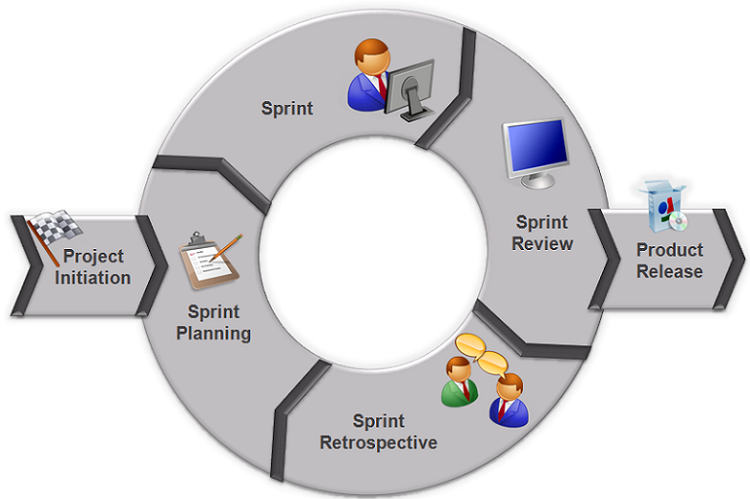
\includegraphics[width=1.2\textwidth]{img/scrum_cicle.png}
\label{fig:scrum_cicle}  
\end{figure} 
\end{landscape}

\section{Factibilidad}
\subsection{Factibilidad Técnica}
Para el desarrollo e implantación del proyecto es necesario contar con los siguientes dispositivos:

\begin{itemize}

    \item Equipo de computo para desarrollo de aplicaciones.
    
    \item MySQL client y MySQL server para bases de datos.
    
\end{itemize}

Así mismo, es necesario contar con los siguientes recursos de software:

\begin{itemize}

    \item Netbeans IDE para desarrollo de aplicaciones
    
    \item Servidor local MySQL.
    
    \item Framework MVC
    
\end{itemize}


\subsection{Factibilidad Operativa}

Este proyecto será elaborado por un estudiante de Ingenieria de Software I, el cual cuenta con el conocimiento previo en las herramientas Netbeans y MySQL.


\subsection{Factibilidad Económica}
El costo del proyecto se presenta con base en: 1) el costo de los equipos requeridos para la elaboración del diseño y desarrollo de los prototipos que requiere el proyecto y 2) el costo de mano de obra de los integrantes. La Tabla \ref{table:Costo-de-Integrantes-del-Proyecto} presenta el costo total de los integrantes del proyecto. La Tabla \ref{table:Costo-de-Recursos} presenta el costo total de los demás recursos requeridos para elaborar el proyecto.   

\begin{table}[ht]
\centering
\caption{Costo de Integrantes del Proyecto}
\label{table:Costo-de-Integrantes-del-Proyecto}
\begin{tabular}{l r c r} \hline
\textbf{Integrante}&\textbf{Valor hora}&\textbf{Horas}&\textbf{Valor total} \\ \hline
Estudiante 1 & \$10.000 & 50 & \$5.000.000 \\ \hline
Estudiante 2 & \$10.000 & 50 & \$5.000.000 \\ \hline
Hector Florez & \$40.000 & 5 & \$2.000.000 \\ \hline \hline
\textbf{Total} & & & \textbf{\$12.000.000} \\ \hline
\end{tabular}
\end{table}

\begin{table}[ht]
\centering
\caption{Costo de Recursos}
\label{table:Costo-de-Recursos}
\begin{tabular}{l c r r} \hline
\textbf{Recurso}&\textbf{Cantidad}&\textbf{Valor Unitario}&\textbf{Valor total} \\ \hline
Equipos de Computo & 2 & \$1.000.000 & \$2.000.000 \\ \hline
Licencia iOS & 1 & \$200.000 & \$200.000 \\ \hline
iPad & 1 & \$700.000 & \$700.000 \\ \hline
Libros & 2 & \$50.000 & \$100.000 \\ \hline
Hosting & 1 & \$100.000 & \$100.000 \\ \hline \hline
\textbf{Total} & & & \textbf{\$0.000.000} \\ \hline
\end{tabular}
\end{table}

\subsection{Factibilidad Legal}
Se utiliza licencia iOS para el desarrollo de aplicaciones en dispositivos móviles.

\section{Cronograma}
La Figura \ref{fig:Cronograma} presenta el cronograma.

\begin{landscape}
\begin{figure}[ht] 
\centering
\caption{Cronograma}
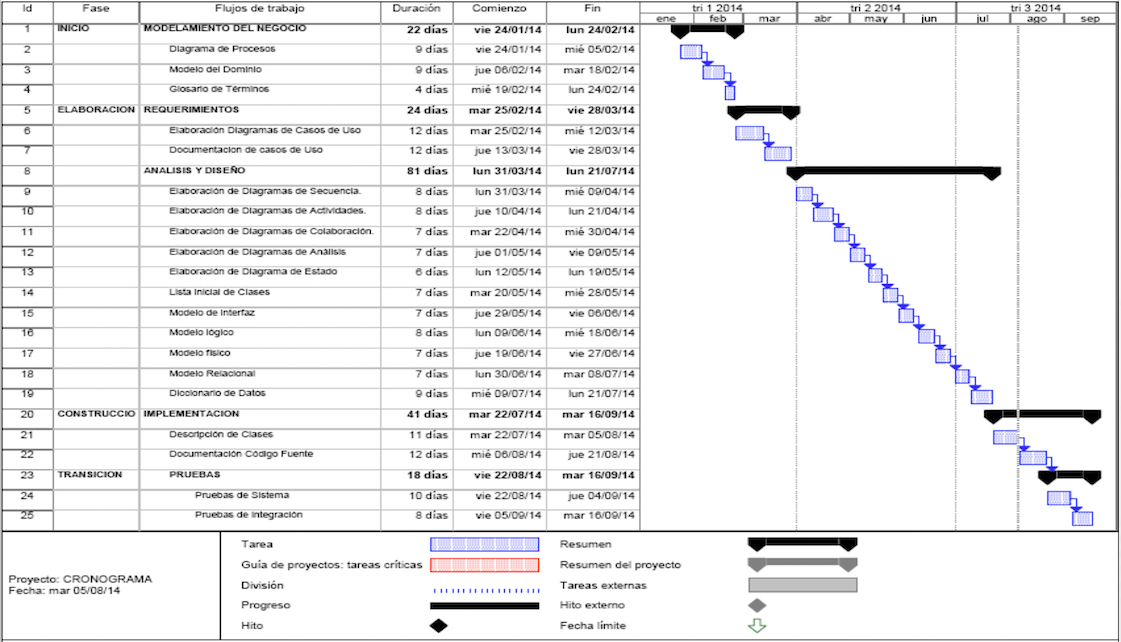
\includegraphics[width=1.2\textwidth]{img/cronograma.png}
\label{fig:Cronograma}  
\end{figure} 
\end{landscape}